%
%
% This is an example LaTeX file which uses the SANDreport class file.
% It shows how a SAND report should be formatted, what sections and
% elements it should contain, and how to use the SANDreport class.
%
% Get the latest version of the class file and more at
%    https://gitlab.sandia.gov/latex/sandreport-latex
%
\makeatletter
\def\input@path{{./sand_report_template}}
\makeatother

\documentclass[12pt,report,justified]{SANDreport}

\usepackage{subcaption}
\usepackage{hyperref}
\usepackage{siunitx}
\sisetup{output-exponent-marker=\ensuremath{\mathrm{e}}}
%\usepackage{draftwatermark}
%\SetWatermarkScale{.5}
%\SetWatermarkText{Sample, contains no OUO}

%if you want to use a clone of the SANDreport standard font,
%  you must install `ebgaramond-maths` package (not included in
%  most standard LaTeX distributions
%\usepackage{ebgaramond} %includes old-style (hanging below the line) numbers.
%\usepackage[lining]{ebgaramond} %if you don't like old-style (hanging below the base line) numbers.
%\usepackage{ebgaramond-maths}
%this command reset the fontfamily setting to use Garamond
%\makeatletter
%\renewcommand{\familydefault}{\ebgaramond@family}
%\makeatother

% Bonus:
% Scientific Notation Command (built-in)

%  This command allows for a standard way to adding units and scientific notation
%    eliminating the need for the constant use of \mathrm and explicitly typing 10^n
%    every time you need a number in scientific notation
%
%  The prototype command is:
%     \sci{mantissa}<exponent>[units]
%  Units will be typeset in mathrm so use standard notation (e.g. [g/cm^3])
%  other forms include:
%     * \sci{mantissa}<exponent>
%     * \sci{mantissa}[units]
%     * \sci{mantissa}
%
%******************* WARNING *********************
%
% Do not be concerned that there are a lot of
% pages marked as 'intentionally left blank'.
% This is required by common-look-and-feel.
%
% DO NOT attempt to change the class to remove
% them! It will not pass common-look-and-feel review
% without the blank pages marked and without
% sections/chapters starting on odd-numbered
% pages.
%
% The class will continue to use the `article`
% style template as default, however,
% `article`-style reports (where the top level
% organizational unit is the `section`,
% not `chapter`) will only be approved for
% for SAND reports under 25 pages.
%
% ************************************************
%
% ---------------------------------------------------------------------------- %
%
% Set the title, author, and date
%


    \title{Peak Map User’s Manual}
     \subtitle{Gamma Matching and Nuclide Library Generation}

	\author{Elliott J. Leonard}

    % There is a "Printed" date on the title page of a SAND report, so
    % the generic \date should generally be empty.
    \date{}


% ---------------------------------------------------------------------------- %
% Set some things we need for SAND reports. These are mandatory
%
\SANDnum{SAND2020-2523 O}
\SANDprintDate{Feb, 2020}

% ---------------------------------------------------------------------------- %
% The following definition does not have a default value and will not
% print anything, if not defined
%
\SANDsupersed{SAND1901-0001}{January 1901}


% ---------------------------------------------------------------------------- %
%
% Start the document
%
\begin{document}
    \maketitle


    % ------------------------------------------------------------------------ %
    % An Abstract is required for SAND reports
    %
    \begin{abstract}
Peak Map is a software tool that allows users to generate nuclide library files for gamma spectroscopy
from a nuclear data reference. This document lays out the necessary information for the
usage of the Peak Map software tool. It includes directions for the correct usage of the software
and information on the algorithms used in the software.
    \end{abstract}


    % ------------------------------------------------------------------------ %
    % An Acknowledgement section is optional but important, if someone made
    % contributions or helped beyond the normal part of a work assignment.
    % Use \section* since we don't want it in the table of context
    %
    \chapter*{Acknowledgement}
    \addcontentsline{toc}{chapter}{Acknowledgement}
Thanks to Michael Enghauser (mwengha@sandia.gov) and Sean Forunier (sdfourn@sandia.gov)
for technical direction and help with testing.


    % ------------------------------------------------------------------------ %
    % The table of contents and list of figures and tables
    % Comment out \listoffigures and \listoftables if there are no
    % figures or tables. %
    \tableofcontents
    \listoffigures
    \listoftables



    % ---------------------------------------------------------------------- %
    % An optional glossary. We don't want it to be numbered
    \chapter*{Acronyms \& Definitions}
    \addcontentsline{toc}{chapter}{Acronyms \& Definitions}
    \begin{description}
	\item[SNL]
	     Sandia National Laboratories
	\item[DOE]
	     United States Department of Energy
	\item[NNSA]
	     National Nuclear Security Administration
          \item[ICRP-107]
	     International Commission on Radiological Protection publication 107 Nuclear Decay Data for Dosimetric Calculations
	\item[keV]
	     Kiloelectonvolts, unit of energy 1000 times the energy needed to move an electron across one volt
	\item[MDA]
	     Minimum Detectable Activity, the point at which a false positive peak identification is setto fixed percentage, typically 5\%
	\item[ROI]
	     Region of Interest, an span of channels on a gamma spectra representing an important region
	\item[CAM]
	     Configuration Access Method, a proprietary file type of storing spectral information used in the Mirion Canberra GENIETM 2000 software package
	\item[CSV]
	     Comma Separated Variable file, a text based file for tabular data were columns are delimited with a comma and rows with new Lines
    \end{description}


    % ---------------------------------------------------------------------- %
    % This is where the body of the report begins; usually with an Introduction
    %
    \SANDmain		% Start the main part of the report

\chapter{Introduction}\label{sec:intro}
Peak Map is a software tool that assists the user with matching unknown peaks from gamma
spectroscopy measurements with corresponding decay signatures and generating nuclide libraries
to be used in gamma spectroscopy analysis. The system uses nuclear data for the International
Commission on Radiological Protection publication 107: Nuclear Decay Data for Dosimetric
Calculations (ICRP-107) as a nuclear data reference however, the system is deigned in such a way
other data references can be used in future releases. Peak matching is done by matching the energy
of a peak to find nuclides with corresponding gamma line signatures and then provides a score.
The score based on the difference in energy of the peak and line, the photon yield of the, and the
half-life of the nuclide in relation to the time between the reference date and the measurement date.
To further increase the confidence of the selection, the other signature lines of the parent, and of the
daughters in equilibrium, are provided with a line match score that is determined by whether the
lines that should be detected have matching peaks in the list. The signature lines and the matching
nuclide information can then be written to a nuclide library file.

\section{About this Manual}\label{sec:about}
This manual is a complete description of the tool and guidance document for users of the system. It
is broken into chapters, the first chapter \hyperref[sec:intro]{Introduction}, is an overview of the tool and this document.
Chapter \hyperref[sec:usage]{Usage} describes how to use the tool to accomplish the goals of the user and Chapter
\hyperref[sec:tech]{Technical} describes the algorithms and equations used within the software.
\hyperref[sec:set_desc]{Appendix~\ref{sec:set_desc}}Appendix A is an
overview of the parameters used in the matching algorithm and \hyperref[sec:install]{Appendix~\ref{sec:install}} provides instructions
on the installation of the software.

    \chapter{Usage}\label{sec:usage}
    This chapter describes the usage and the the complete functionality of the tool. It is broken into
    the menus available to the user. The terminology is as follows:
    \begin{itemize}
        \item Left Click - Use the mouse left button
        \item Right Click - Use the right mouse button
        \item Navigate - Move through the menus as directed, using the mouse or keyboard (ALT+letter)
        \item Select - Click on a row
        \item Selected - Highlighted row
        \item Multi-Select - Select multiple rows by using the left click while holding the Control key (CTRL) or the Shift Key (SHIFT)\
        \item Drag and Drop - Left click and hold on a file, move the mouse over the Peak Map tool, and release the mouse button
    \end{itemize}
The tool has two modes, Matching Mode and Library Mode. The former is for matching a list of
peaks to signature lines and nuclides then writing a nuclide library file. The latter, is for entering
nuclides and writing them and the signature lines to a nuclide library file. Library mode is useful
for quickly creating nuclide libraries of known nuclides. The tool always opens in the matching
mode by default, but can be switched to the library mode by navigating to \textbf{Settings}
\(\rightarrow\) \textbf{Mode} or and selecting the desired mode or pressing F5 to toggle between the
two modes. The window will toggle between \hyperref[fig:main_window]{Figure~\ref{fig:main_window}}
and \hyperref[fig:lib_mode]{Figure~\ref{fig:lib_mode}}, display a subset of the columns in the
remaining grids, and hiding peak input information.

Irespective of the mode, the window containts three grid views, one on the left for the peaks in
matching mode or written nuclides in library mode and two on the top and bottom of the right side
of the window. The upper right grid displays the found nuclides from either a matching line or searched
nuclide. The bottom right grid shows all the characteristic lines from the selected nuclide and any
daughters in equilibrium with the nuclide. This grid can be filtered by expanding the the Line Filters
which can include/exclude Daughter Lines, x-Rays, Gamma-Rays, provide a minimum yield and a window the
line energies. The strip at the bottom of the screen presents information about loaded spectra/peak
files, and the nuclide library file that is being written.
%Between the two grids is the line match score or the score determined by the number of detectable lines that are associated with peaks.

\section{Matching Mode}\label{sec:match_mode}
\begin{figure}[h]
    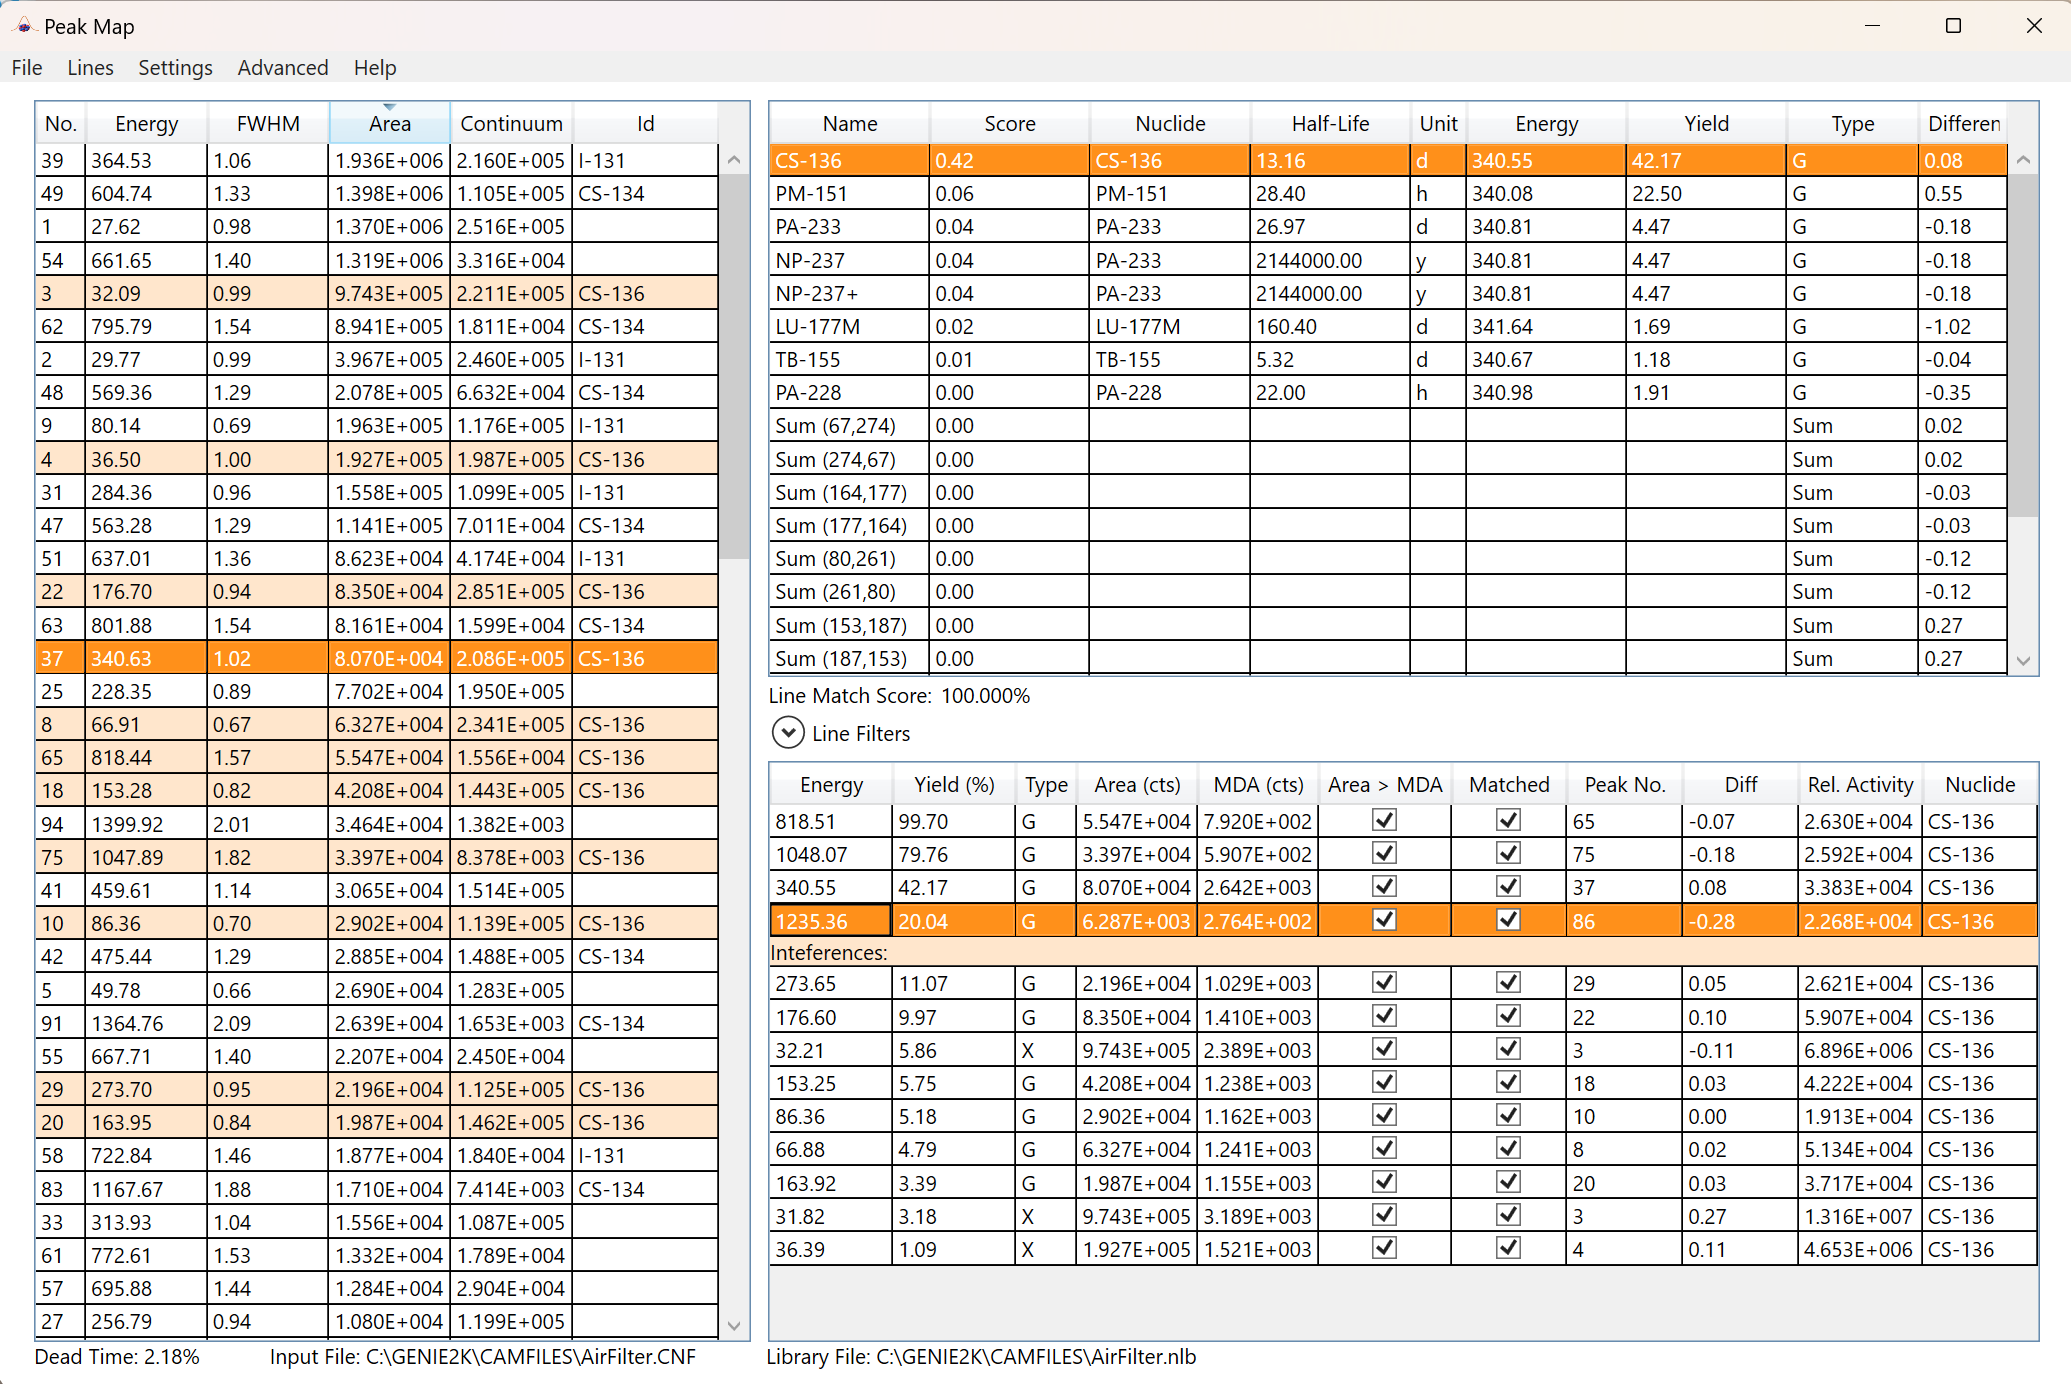
\includegraphics[width=0.85\textwidth]{MainWindow.png}
    \centering
    \caption{Peak Map window in matching mode performing peak matches.}
   \label{fig:main_window}
\end{figure}

The columns in the peaks grid are as follows:
\begin{itemize}
    \item \textbf{No.} - An identification number for the peak.
    \item \textbf{Energy} - The energy of the peak centroid in kiloelectronvolts (keV).
    \item \textbf{FWHM} - The Full width at half maximum of peak in keV.
    \item \textbf{Area} - The number of counts in the peak.
    \item \textbf{Continuum} - The number of counts in the continuum under the peak.
    \item \textbf{Id} - The nuclides, separated by a comma, matched to the peak.
\end{itemize}

The columns in the nuclides grid are as follows:
\begin{itemize}
    \item \textbf{Name} - The nuclide to be associated with matched lines or decay chain (see \hyperref[sec:decay_chain]{Appendix~\ref{sec:decay_chain}} for a discussion on the decay chains).
    \item \textbf{Score} - The score associated with the match of the nuclide to the selected peak.
    \item \textbf{Nuclide} - The actual nuclide that emits the characteristic line.
    \item \textbf{Half-Life} - The half-life of the nuclide listed in the \textbf{Name} column.
    \item \textbf{Unit} - The unit of half-life.
    \item \textbf{Energy} - The characteristic energy of the line matched with the peak in keV.
    \item \textbf{Yield} - The photon yield, in percent, of the matched line from the nuclide in the \textbf{Name} column. This includes nuclide branching ratios if applicable.
    \item \textbf{Type} - Emission type: \textbf{X} for x-rays, \textbf{G} for gamma rays.
    \item \textbf{Diff} - The Difference between the peak centroid energy and the characteristic energy of the matched line in keV.
\end{itemize}

The column in the lines grid are as follows:
\begin{itemize}
    \item \textbf{Energy} - The energy of the characteristic line in keV.
    \item \textbf{Yield} - The photon yield, in percent, of the characteristic line in the \textbf{Name} column. This include nuclide branching ratios if applicable.
    \item \textbf{Type} - Emission type: \textbf{X} for x-rays, \textbf{G} for gamma rays.
    \item \textbf{Efficiency} - The detection efficiency, in percent, at the energy of the characteristic line. This will be zero if there is no efficiency information.
    \item \textbf{Area} - The expected area of a peak, based on the selected peak, for this line.
    \item \textbf{MDA}- The minimum area (\(95^{\text{th}}\) confidence interval) a peak would need to have to be detected.
    \item \textbf{Matched} - Checked if a peak was found that matches to the line.
    \item \textbf{Peak No.} - The identification number of the matched peak, blank if Matched is unchecked.
    \item \textbf{Diff} - The difference between the matched peak centroid and the line energy in keV. Blank if the \textbf{Matched} is unchecked.
    \item \textbf{Rel. Activity} - The expected activity, based on the selected peak, of this line relative to the other lines. Blank if the \textbf{Matched} is unchecked.
    \item \textbf{Name} - Library Mode only. The name of the nuclide emitting the line.
\end{itemize}

Matching Mode as shown in \hyperref[fig:main_window]{Figure \ref{fig:main_window}} allows for
increasing complexity and more sophistication in the matching and scoring algorithms depending
on the availability of information. The minimum amount of information required is a single peak
centroid energy. The tool will accept various peak input formats (details in
\hyperref[sec:peak_inp]{Peak Inputs \ref{sec:peak_inp}}); but the input data fits into three
categories: peak information, time information, and efficiency calibration Information. Peak
Information includes the location of the peak (\textit{centroid/energy}), and the size
(\textit{area}) and the underlying continuum (\textit{Continuum}). These parameters can be
entered into the peaks grid manually one by one. Time information includes the length of the count
(\textit{Acquisition time}), the time elapsed from the time the acquisition began
(\textit{Start Time}), and the time the sample was collected (\textit{Sample Time}). The time
parameters are used in \hyperref[sec:score]{Nuclide Scoring} to help filter out short lived
nuclides that may be impossible to detect given the span of time between \textit{sample time} and
\textit{start time} and the half-life of the nuclide. These parameters are entered through the
\hyperref[sec:set_menu]{Settings Menu} or loaded through a compatible input file. Efficiency
calibration information allows for the \hyperref[sec:sec:ln_score]{Line Scoring} and comparative
peak calculations to occur (\textit{area, MDA,} and \textit{relative activity}) as well as the
efficiency at the line energy. The calibration curve model, order of polynomial and efficiency
measurements (\textit{Energy, Efficiency, Efficiency Uncertainty}) can be entered through
\hyperref[sec:set_menu]{Settings Menu} or loaded though a compatible input file. There are three
available models: Linear (\hyperref[sec:eq:eff_lin]{Equation \ref{eq:eff_lin}}), Natural
(\hyperref[eq:eff_dul]{Equation \ref{eq:eff_dul}}), and Empirical
(\hyperref[eq:eff_emp]{Equation \ref{eq:eff_emp}}). The calibration curve is computed
(\hyperref[eq:eff_coeff]{Equation \ref{eq:eff_coeff}}) on-the-fly and will be recalculated when any
of the calibration settings are changed.

\subsection{Tips for Matching}\label{sec:match_tips}
\begin{itemize}
    \item The first nuclide is not always the best match because the line match score is not part of the nuclide
    score. It is therefore best to select several nuclides before deciding.
    \item Start at high energy peaks and work toward low energy. Many low energy peaks (less than 80 keV) are
    x-rays from the nuclides that also have more distinct gamma emissions in the higher energies.
    \item Start with the largest peaks, the matched nuclides will likely have other lines reducing the effort
    needed.
    \item Avoid jumping around to different peaks, finish with one peak before moving on.
    \item If the efficiency calibration is a good representation, the relative activity across the energy lines
    should be uniform for a correctly identified nuclide.
    \item If the camparitive analysis is valid, clicking on a line in the lines grid can expose potential identified
    interferences.
    \item If a line peak has a relative activity that is different from the others, it might be an interference
    with another nuclide.
    \item Look for peak areas that should be above the MDA and determine why they were not found.
    \item Enter as much information about the spectrum as possible, information unlocks the more sophisticated
    matching tools.
    \item Ignore the comparative analysis if there are no peak areas or efficiency calibration.
\end{itemize}
The nuclide and lines can be written to a nuclide library for use in vendor supplied gamma spectroscopy software.
To generate or append a library, a library must be loaded. This can be done from, the
\hyperref[sec:file_menu]{File Menu} menu. Selecting \textbf{New\ldots} will generate a new library file or overwrite
the library if a file with the same name exists. \textbf{Open]\ldots} will append the nuclides and lines to the
selected file. Both options will open a window where to browse for a file or a save location. Three file types are
available: .nlb, .cnf, .tlb. The .nlb and .cnf files are CAM file types to be used in the \(\text{GENIE}^\text{TM}\)
2000 software package. The third (tlb) is a text based library that can be opened with any text editor. Once the
file is ready to be written, the file name will appear in the status strip and the write options in
\hyperref[sec:line_menu]{Lines Menu} will become active. To write the lines, determine how they should be written
and select the appropriate option from the \hyperref[sec:line_menu]{Lines Menu}. The options are as follows:
\begin{itemize}
    \item \textbf{Selected} - Write the highlighted lines that have been selected in the Lines Grid
    \item \textbf{Matched} -  Write only the lines that have matching peaks, delineated by a check mark in the
    \textbf{Matched} column. \textit{Available in Matching Mode only.}
    \item \textbf{All} - Write every visible line in the Lines Grid.
\end{itemize}

Every line, independent of the option chosen, will be written to the selected nuclide. Lines from daughters
in equilibrium can be associated with their parent or a decay chain
(\hyperref[sec:decay_chain]{Appendix \ref{sec:decay_chain}}) by selecting the desired
nuclude in the nuclide grid. \textbf{Note:} Attributing daughter lines with parents will write the lines to the
parent nuclide, (with the parent half-life) and the line yield will be adjusted for branching ratios.

The key line for the nuclide is determined by finding the line with the largest abundance that does
not have any lines from other nuclides that are within the interference band. The symmetrical band
can be adjusted with the \textbf{Key Line Interference} parameter described in
\hyperref[sec:set_desc]{Appendix \ref{sec:set_desc}} section:
\hyperref[itm:ky_inf]{Key Line Interference}.

\subsection{Peak Inputs}\label{sec:peak_inp}
\begin{table}[h!]
    \centering
    \caption{Peak input options and the class of data that is automatically or manually loaded}
    \begin{tabular} {r|c|c|c}
        \hline
        Input Type & Peak Info. & Time Info. & Efficiency Cal. \\
        \hline
        CAM & Auto. & Auto. & Auto.\\
        CSV & Auto. & Manual & Manual \\
        User & Manual & Manual & Manual \\
        \hline
    \end{tabular}
   \label{tab:peak_inp}
\end{table}

There are several ways to import peak and spectral information.
\hyperref[tab:peak_inp]{Table \ref{tab:peak_inp}} shows the available inputs and
the data that is automatically and manually loaded. A Mirion Canberra \(\text{GENIE}^{\text{TM}}\) 2000
Configuration Access Method (CAM) file can be loaded. This will load all the peak information, time
information and calibration information, if available in the file. The peaks must have already been located
and areas determined before the file is loaded. Continuum information is read directly from the spectrum so
the MDA calculations are complete. Another way to load data into the tool is to import a PeakEasy ROI Data
Comma Separated Value (CSV) file. This will have all the peak information, but efficiency calibration and time
information will need to be loaded manually. The PeakEasy file type uses linear interpolation between peaks to
determine the continuum, which is a degradation of accuracy in the MDA from the CAM file but serves as a
good approximation. The final method of entering data is completely manual; every piece of information must be
entered manually and there is no way of determining the continuum so only the MDA calculations for found peaks
will be accurate, if peak area was entered. An array of peak energies can be pasted into the peaks grid with
typical Windows paste operations. The other input file types can be dragged and dropped into the window or open
through the \hyperref[sec:file_menu]{File Menu} \(\rightarrow\) \textbf{Input\ldots} CAM files can take a few seconds
to load, but once the file is loaded the peaks will appear in the peaks grid, and the input file name will be
displayed in the status strip at the bottom of the window.

\section{Library Mode}\label{sec:libMode}
\begin{figure}[h]
    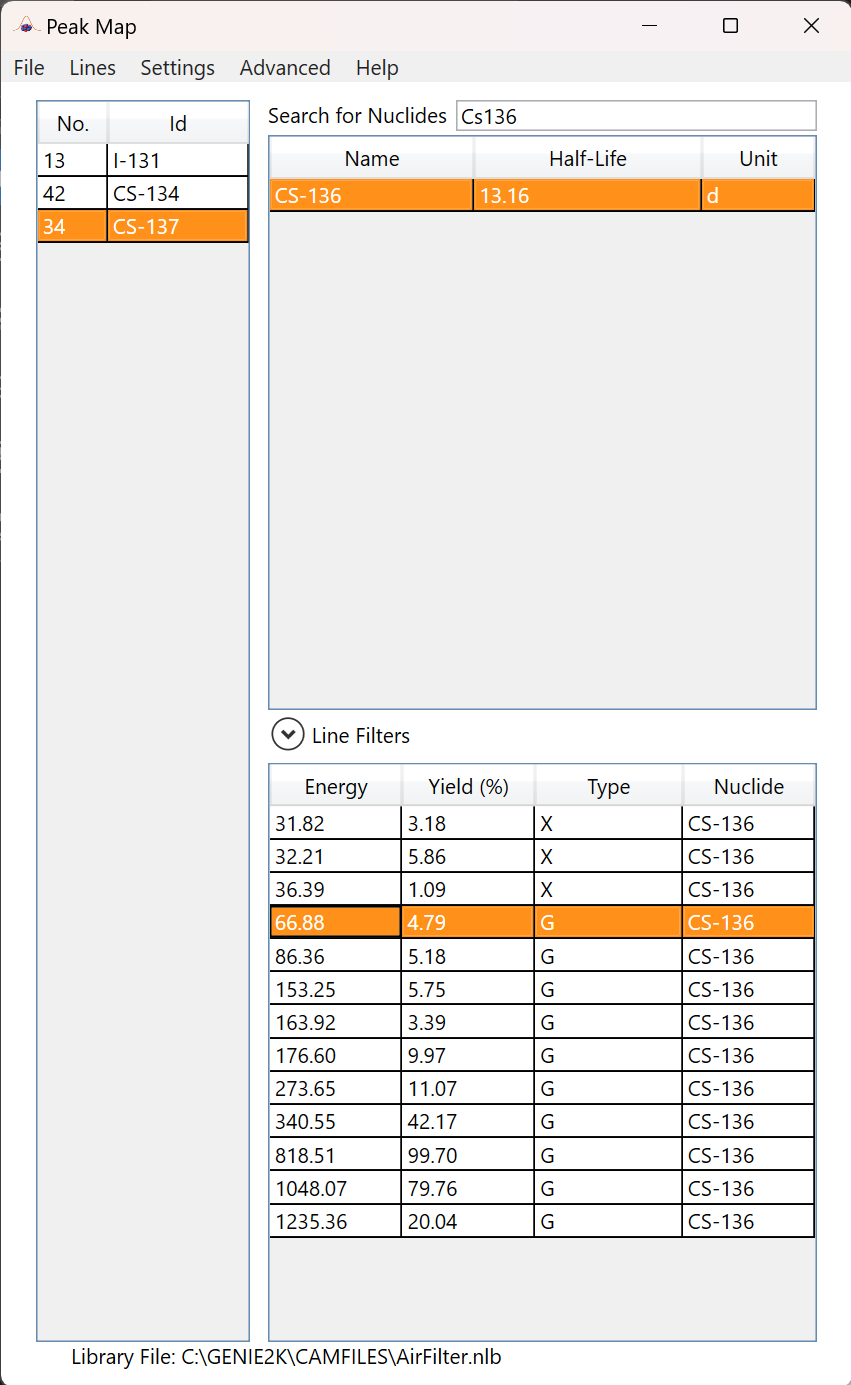
\includegraphics[width=0.3\textwidth]{LibraryMode.png}
    \centering
    \caption{Peak Map window in library Mode}
   \label{fig:lib_mode}
\end{figure}
Library Mode (\hyperref[sec:fig:lib_mode]{Figure \ref{fig:lib_mode}})
allows for the searching of nucluide names and the displaying and library generation of the resultant nuclides and
lines. Selecting library mode from the \hyperref[sec:set_menu]]{Settings Menu} or pressing F5 toggles between library
and matching mode. Typing a nuclide (e.g. Cs137, or CS-137, 137cs) in the search bar will search for that nuclide
and its daughters in equilibrium. An incomplete entry can also be entered, fore example, only the chemical symbol
or and isomer number. The former will find all isotopes of the chemical entered chemical symbol, and the former
all the isomers of the entered number and the associated daughters. If the entered value is part of a decay chain
(\hyperref[sec:decay_chain]{Appendix~\ref{sec:decay_chain}}) the entire chain will be
retrieved and displayed. Clicking on the nuclide in the grid will display all the associated lines with that nuclide,
and daughters if applicable. The lines from the daughters can be toggled on or off from the
\hyperref[sec:line_menu]{Lines~Menu} or right clicking and clicking \textbf{show daughter lines}. The lines can be
written to the library in the same as in the \hyperref[sec:match_mode]{Matching Mode} and the nuclides added will
show up in the left most pane. Nuclides and all their lines can be removed by selecting the nuclides to remove and
right clicking and selecting \textbf{Clear Selected}. \textbf{Clear Current Row} will delete just the row that was
right-clicked on, and \textbf{clear Matches} will clear the whole table.
    \chapter{Menu Navigation}\label{sec:menu}
      \section{File Menu}\label{sec:file_menu}
      \section{Lines Menu}\label{sec:line_menu}
      \section{Settings Menu}\label{sec:set_menu}
      \section{Advanced}\label{sec:adv_menu}
      \section{Help Menu}\label{sec:help_menu}

    \chapter{Technical}\label{sec:tech}
The following algorithms are used to perform all the calculations in the tool. They are provided
for clarity, transparency and to allow advanced users to tweak the parameters to fit their specific
needs. There are two main categories of algorithms, one for matching and one for nuclide library
generation.
      \section{Matching}\label{sec:match}
The matching algorithms are used in \hyperref[sec:match_mode]{Matching Mode} to assist the user in
determining which nuclides are present in a set of peaks. The correctness of a matched is judged by
two scores: the nuclide score and the line score. Both scores depend on the amount of information
in the input file. See \hyperref[sec:peak_inp]{Peak Inputs} for more information on the data from the
various inputs.

      \section{Scoring}\label{sec:score}
The score is a series of penalties ascribed to the selected nuclide (\textbf{Name} column) in the Nuclides
Grid based on the number of elapsed half-lives, the deviation of the peak centroid from the matched
line energy, and the yield of the matched line. The line score is a metric of the number of lines
that should have been detected that have a matching peak.

        \subsection{Nuclide Scoring}\label{sec:nuc_score}
The nuclide score begins at a value of 1.0 and is assigned a penalty for elapsed half-lives, deviation
of peak centroid line energy and sum peak, and the yield of the matched line with the subscripts
for \(S\) in \hyperref[eq:nuc_score]{Equation \ref{eq:nuc_score}} \(k = T_{1/2},D, y, SP\) respectively.
\begin{equation}
    S_N = 1.0 \cdot \prod_{k=0}^{3} s_k, i: \left\{T_{1/2},D,Y,SPl\right\}
   \label{eq:nuc_score}
\end{equation}
The subscript \(T_{1/2}\) represents the penalty for the number of half-lives \(\left(T_{1/2}\right)\) that have elapsed
during the start of \hyperref[itm:time_acq]{Acquisition Time} and the \hyperref[itm:time_smp]{Sample Time}
\(\left( \Delta T\right)\) and is shown in \hyperref[eq:hl_score]{Equation \ref{eq:hl_score}}. The severity of the
penalty can be adjusted using the \hyperref[itm:hl_const]{Half-Life Constant} \(\left(C_{1/2}\right) \).
\begin{equation}
S_{T_{1/2}} = \exp{\left[ C_{1/2} \cdot \left( \frac{\Delta T}{T_{1/2}} \right) \right]}
\label{eq:hl_score}
\end{equation}
The score is further reduced by measurement between the peak centroid and the line energy from
the reference \(\left( \Delta T\right)\). The line search tolerance  \(\left( \delta _E\right)\) which is set to
the Peak FWHM, if available, and the line yield is also accounted for in this determination. The
product of the  \(\Delta T\) and \( \delta _E\) is squared to ensure it is always positive and the \(S_D\)
acts as a penalty. Just as with the half-life penalty the severity can be adjusted with a constant
\hyperref[itm:ln_dev_const]{Line Deviation Constant} \(\left(C_D \right)\). For nuclides, the deviation penalty
as expressed in \hyperref[eq:hl_score]{Equation \ref{eq:hl_score}} accounts for yield  \(\left( y_r \right)\) of
 the reference line. For escape peaks and sum peaks, the yield is excluded as it is strongly dependent on
the counting geometry and such calculations are unnecessary for these purposes.
\begin{equation}
S_D = \exp{\left[ C_D \cdot \frac{\left(\delta_E \cdot \Delta E \right)^2 \cdot y}{100} \right]}
\label{eq:dev_score}
\end{equation}
The lines that appear in a spectra are likely the most abundant lines from the nuclide. To account for
this the score if further reduced by the yield penalty (\hyperref[eq:yld_score]{Equation \ref{eq:yld_score}}).
The score is simply multiplied by the fractional yield of the reference line \(\left( y_r\right)\), linearly
reducing the score. The half-life penalty (\hyperref[eq:hl_score]{Equation \ref{eq:hl_score}}) mirrors the
decay equation, a small penalty for few half-lives and a very large penalty for many half-lives. The deviation
penalty (\hyperref[eq:dev_score]{Equation \ref{eq:dev_score}}) is also a exponential to severely penalize
lines that approach the search tolerance \(\left( \delta _E \right)\).
\begin{equation}
S_y = \frac{y_r}{100}
\label{eq:yld_score}
\end{equation}
Sum peaks require at least three peaks to be present in a spectrum for the possibility of sum peaks
to arise. Furthermore, the chance of multiple sum peaks is greatly reduced if the two peaks with
the largest area do not sum a peak in the peaks grid. The accounting for these facts is done with
the sum peak score \(\left( S_{SP} \right)\) expressed in \hyperref[eq:sp_score]{Equation \ref{eq:sp_score}}
which acts as cutoff essentially removing the possibility of sum peaks if there are not three peaks and the
largest peaks do not sum to a peak in the spectrum.
\begin{equation}
S_{SP} =
\begin{cases}
P, \text{there are less than 3 peaks} \\
P, \text{there is no peak that matches the energy sum of the 2 largest peaks} \\
1, \text{otherwise}
\end{cases}
\label{eq:sp_score}
\end{equation}
The \hyperref[itm:sm_peak_pen]{Sum Peak Penalty} is an adjustable parameter and as with the other
penalty constants whichallows the user to finely tune the nuclide scores within a session of matching.


\subsection{Line Scoring}\label{sec:ln_score}
Once a nuclide is selected in the nuclides grid the line score is generated and represented as a
percent. This score is a measure of the lines that were found in the peaks grid against the lines
that should have been found. To determine which lines should have been found, an efficiency
calibration is required, as well as a measurement of continuum where MDA can be determined.
For the ith line attributed to the nuclide, the Minimum detectable activity \( \left(MDA_i\right) \),
efficiency at
the line energy \(\left(e_i\right)\), and the activity \(\left( a_i\right)\) relative to the reference line (denoted with subscript \(r\)) is
calculated using the \hyperref[sec:comp_calcs]{Comparative calculations}. The reference line is the line found that matches
the highlighted peak in the peaks grid. The denominator in \hyperref[eq:line_score]{Equation \ref{eq:line_score}} is all the lines that should
be detected with (di) indicating if it should have been detected. The numerator is the number of
lines found in the spectra. The severity of the penalty can be scaled with \(\left(C_L\right)\) and is described in
\hyperref[sec:set_desc]{Appendix \ref{sec:set_desc}} section: \hyperref[itm:sm_peak_pen]{Unmatched Line Constant}. It is possible of the \hyperref[eq:line_score]{Equation \ref{eq:line_score}} to exceed 100\% if
lines that should not have been detected were. It might indicate and interference.
\begin{equation}
S_L = C_L \cdot \frac{\sum_i^N y_i \sqrt{\epsilon _i}}{\sum_i^N \delta _i \cdot y_i \sqrt{\epsilon _i}} \cdot 100
\label{eq:line_score}
\end{equation}

\subsection{Comparative Calculations}\label{sec:comp_calcs}
The comparative calculations are required for the \hyperref[sec:ln_score]{Line Scoring} to be accurately calculated. The
calculation of MDA \hyperref[eq:rel_mda]{Equation \ref{eq:rel_mda}} and relative activity \hyperref[eq:rel_act]{Equation \ref{eq:rel_act}} are required for the determination of \(\delta _i\) in \hyperref[eq:line_score]{Equation \ref{eq:line_score}}. The MDA is calculated using the Currie method at the 95\% confidence level, where \(\mu _i\) is the continuum counts at the energy of the \(i^{th}\) line of the selected nuclide.
\begin{equation}
\text{MDA} = 2.71 + 2 \sqrt{\mu _i}
\label{eq:rel_mda}
\end{equation}
The relative activity is based off the activity of the reference line \(\left(A_r\right)\). It requires the efficiency
and yield of both the reference line (\(\epsilon _r \) and  \(y_i\), respectively), and the efficiency and yield of the \(i^{th}\)
line.
\begin{equation}
A_i = \frac{A_r \cdot \epsilon _i \cdot y_i}{\epsilon _r \cdot y_r}
\label{eq:rel_act}
\end{equation}

\subsubsection{Efficiency}\label{sec:eff}
An efficiency calibration is essential of the determination of the relative activity (\hyperref[eq:rel_act]{Equation \ref{eq:rel_act}}).
Following the convention in gamma spectroscopy the efficiency calibration is a curve regression
fitted to several peak areas across the energy range as compared to a known standard. There
are three available models: Linear found in \hyperref[eq:eff_lin]{Equation \ref{eq:eff_lin}}, Natural in \hyperref[eq:eff_dul]{Equation \ref{eq:eff_dul}} and Empirical
\hyperref[eq:eff_emp]{Equation \ref{eq:eff_emp}}.
\begin{equation}
\log{\left( \epsilon \right)} = \sum_{i=-1}^M b_i \cdot \frac{1}{E}^i
\label{eq:eff_lin}
\end{equation}

\begin{equation}
\ln{\left( \epsilon \right)} = \sum_{i=0}^M b_i \cdot {\left[\ln{{\left(E\right)}}\right]}^i
\label{eq:eff_dul}
\end{equation}

\begin{equation}
\ln{\left(\epsilon \right)} = \sum_{i=0}^M b_i \cdot \left[ \frac{0.5 \cdot \left( E_0 + E_H\right)}{E} \right]^i
\label{eq:eff_emp}
\end{equation}
The curve allows for an energy \(E\) and the fit of the curve is controlled by the fitting coefficients
\(\left(b_i\right)\) can be entered in the Spectral Settings menu, described in \hyperref[sec:set_desc]{Appendix \ref{sec:set_desc}} section:
\hyperref[itm:cal_coeff]{Calibration Parameters}.

The efficiency curves are calculated from the efficiency measurements loaded from the spectral file
or entered manually in the \hyperref[itm:eff_pts]{Efficiency Points}. The coefficients \(\left( b_i \right)\) are determined by using weighted
least squares methodology. It is also known that the efficiency measurement is associated with
uncertainty, and logically, measurements of high uncertainty should contribute less to the solution.
Thus, a weight, that is a function of the uncertainty is applied to both sides of the efficiency
equation.
\begin{equation}
w_j = \left( \frac{\epsilon}{\sigma_{\epsilon}} \right)^2
\label{eq:eff_wgt}
\end{equation}
Given \(N\) Efficiency Points and a order of \(M\) the \hyperref[eq:eff_lin]{Equations \ref{eq:eff_lin}, \ref{eq:eff_dul} and, \ref{eq:eff_emp}} can be rewritten in in matrix form.
\begin{equation}
\mathbf{A} \overrightarrow{b} \overrightarrow{w} = \overrightarrow{\epsilon} \overrightarrow{w}
\label{eq:mat_eff}
\end{equation}
For simplicity and clarity, the weights will be rolled into the \(\mathbf{A}\) and \(\overrightarrow{\epsilon}\). Since the efficiencies
\(\left(\overrightarrow{\epsilon}\right)\) are measured values there is no solution to \hyperref[eq:mat_eff]{Equation \ref{eq:mat_eff}} we must find a estimated solution \(\left(\overrightarrow{b^*}\right)\) that minimizes the \hyperref[eq:wt_mat_eff]{Equation \ref{eq:wt_mat_eff}}.
\begin{equation}
\| \overrightarrow{\epsilon} - \mathbf{A}\overrightarrow{b^*} \|
\label{eq:wt_mat_eff}
\end{equation}
This is achieved using the least squares method, where both sides of \hyperref[eq:mat_eff]{Equation \ref{eq:mat_eff}} are multiplied by
transpose of \(\mathbf{A}^T\) and the result is inverted to give \(\overrightarrow{\epsilon }\). The solution is given in \hyperref[eq:eff_coeff]{Equation \ref{eq:eff_coeff}}.
\begin{equation}
\overrightarrow{b^*} = \mathbf{A}^T\overrightarrow{\epsilon} \cdot \left( \mathbf{A}^T \mathbf{A} \right)^{-1}
\label{eq:eff_coeff}
\end{equation}


\section{Library}\label{sec:library}
The generation of nuclear data libraries for use in gamma spectroscopy software requires the calculation
of uncertainty because ICRP-107 does not list uncertainties. The tool will also combine
lines that may be unreasonable in a spectrum. The limit on how close peaks must be to be combined
are outlined in \hyperref[sec:set_desc]{Appendix \ref{sec:set_desc}} section: \hyperref[itm:res_lim]{Resolution Limit}. Line combination can be disabled
in \hyperref[sec:set_desc]{Appendix \ref{sec:set_desc}} section: \hyperref[itm:ln_combo]{Line Combination} if it is not desired. Also the tool will ask the user to
confirm the combination of lines each time it detects combination a situation.

\subsection{Uncertainty}\label{sec:unc}
The uncertainty for any number is assigned as half the last digit of precision. ICRP-107 lists
energies in MeV and yields in gammas per decay in scientific notation with six digits. Therefore,
the uncertainty can be six orders of magnitude smaller than the listed value. The uncertainty is 0:5
of the last non-zero significant digit, the median between the precision of the listed value. This
sample logic applies to half-life values, which are listed as floats in ICRP-107.

\subsection{Combining Lines}\label{sec:comb_lines}
No gamma spectroscopy technology has perfect charge collection, and by continuation the peaks
are not infinitely thin. As a result, there is a possibility that lines from a single nuclide may need
to be combined if they are smaller than the resolution of the system used to collect the spectrum.
This is particularly prevalent within the x-ray region of the spectrum. The energy of the combined
peak is simply the yield (\(y_i\)) weighted average of the line energies (\(E_i\)) over the number of peaks to
combine (\(N\)) and is given in \hyperref[eq:ave_E]{Equation~\ref{eq:ave_E}}.
\begin{equation}
\bar{E} = \frac{\sum^{N}_{i} E_i \cdot y_i}{\sum^{N}_{i}y_i}
\label{eq:ave_E}
\end{equation}

The uncertainty in the energy of the combined peak (\( \sigma _{\bar{E}}\)) is the weighted average standard deviation
in the line energies. \hyperref[eq:ave_E_sig]{Equation~\ref{eq:ave_E_sig}} is used to determine the uncertainty in the combined line energy.
\[
\sigma_{\bar{E}} = \sqrt{\frac{\sum^{N}_{i} y_i \left( E_i - \bar{E} \right) ^2}{ \frac{N-1}{N} \cdot \sum^{N}_{i} y_i}}
\label{eq:ave_E_sig}
\]
The yield of the newly combined peak is just simple addition of the yields. It is possible for this
yied to exceed 100\% if the nuclear decay structure has many high yield instantaneous decays.
\hyperref[eq:ave_yld]{equation \ref{eq:ave_yld}} is used for the addition.
\[
\bar{y} = \sum^N_i y_i
\label{eq:ave_yld}
\]
Uncertainty in the combined yield (\( \sigma _{\bar{y_i}} \)) in \hyperref[eq:ave_yld_sig]{equation~\ref{eq:ave_yld_sig}} is just propagation of errors of the yield
uncertainty as determined in the Uncertainty section.
\[
\sigma_{\bar{y}} = \sqrt{\sum^N_i \left( \sigma_{y_i} \right) ^2}
\label{eq:ave_yld_sig}
\]


    % ---------------------------------------------------------------------- %
    % References
    %
    % Comment \nocite{*} to not cite every reference in your master library,
    % just the ones cited in this document.
    \nocite{*}

    \bibliographystyle{plain}
    \bibliography{SANDExample}


    % ---------------------------------------------------------------------- %
    %
    \appendix
    \chapter{Settings Description}\label{sec:set_desc}

\section{Matching}
\begin{center}
{\large \textbf{Algorithm Settings}}
\end{center}
\begin{description}
\item[Enable Half-Life Score]\label{itm:hl_score} \hfill \\
\textbf{Default:} True. Turn on or off the half life scoring. May be necessary if a very large amount
of a short lived nuclide may be present.
\item[Half-Life Constant]\label{itm:hl_const} \hfill \\
\textbf{Notation:} \( C_{1/2}\) \textbf{Default:} -0.0051. The constant to adjust the severity of the half-life penalty.
centroid to line energy penalty.
\item[Line Deviation Constant]\label{itm:ln_dev_const} \hfill \\
\textbf{Notation:} \( C_D\) \textbf{Default:} -0.5. The constant to adjust the severity of the deviation of peak
centroid to line energy penalty.
\item[Sum Peak Penalty]\label{itm:sm_peak_pen} \hfill \\
\textbf{Notation:} \( P\) \textbf{Default:} 0.1. The penalty assigned to possible sum peaks when summing is
not likely.
\item[Unmatched Line Constant]\label{itm:um_line_const} \hfill \\
\textbf{Notation:} \( C_L\) \textbf{Default:} 1.0 The constant to adjust the severity of an unmatched in the Line Match score.
\end{description}

\begin{center}
{\large \textbf{Limit Settings}}
\end{center}
\begin{description}
\item[Parent/Daughter Half-Life Ratio]\label{itm:pd_hl_ratio} \hfill \\
\textbf{Default:} 1.0. The ratio of the parent’s half-life to the daughter’s to serve as indication if the
pair are in equilibrium and will be added as a pair or a single nuclide.
\item[Score Limit]\label{itm:score_lim} \hfill \\
\textbf{Default:} 0.001. The cutoff for lowest score to be included in the nuclides grid.
\item[Yield Limit]\label{itm:yld_lim} \hfill \\
 \textbf{Default:} 0.1. The smallest line yield to be included in the search or lines grid.
\end{description}


\section{Library}
\begin{center}
{\large \textbf{Line Combination Settings}}
\end{center}
\begin{description}
\item[Line Combination]\label{itm:ln_combo} \hfill \\
\textbf{Default:} True. Turn on or off the line combination during library generation.
\item[Resolution Limit]\label{itm:res_lim} \hfill \\
\textbf{Default:} 0.5. The largest difference between line energies in keV to still be considered
individually resolved.
\item[Key Line Interference]\label{itm:ky_inf} \hfill \\
 \textbf{Default:} 3.0. The symmetrical band limit in keV where there may be and interference and to
not set as the key line for that nuclide
\end{description}
\section{Spectral}

\begin{center}
{\large \textbf{Calibration}}
\end{center}
\begin{description}
\item[Calibration Model]\label{itm:cal_model} \hfill \\
\textbf{Default:} Linear. The type of curve fit to use to model the efficiency of the count.
\item[Calibration Parameters]\label{itm:cal_coeff} \hfill \\
\textbf{Default:} \( \left\{ \num{1.0e-4}, \num{1.4e-17}, \num{-8.7e-19}  \right\}\). The fitting constants for the
calibration model. The default is a constant calibration of 100\% efficiency across the entire
spectrum.
\item[Order]\label{itm:cal_order} \hfill \\
 \textbf{Default:} 5 or 2. The number of terms in the calibration equation. Changing this will recalculate
the calibration parameters.
\item[Efficiency Points]\label{itm:eff_pts} \hfill \\
 \textbf{Default:} \(
\left\{ \begin{matrix}
20.0 & 0.9999999999999 & 0.000000000005 \\
1510 & 0.9999999999999 & 0.000000000005  \\
3000 & 0.9999999999999 & 0.000000000005
 \end{matrix}
 \right\} \) \\
The efficiency measurements used to determine the efficiency equation
\end{description}

\begin{center}
{\large \textbf{Time}}
\end{center}
\begin{description}
\item[Acquisition Time]\label{itm:time_acq} \hfill \\
The date and time the count was started.
\item[Count Time]\label{itm:time_cnt} \hfill \\
The time the sample was counted in seconds.
\item[Sample Time]\label{itm:time_smp} \hfill \\
The date and time the sample was collected or reference date or time. The difference between
\hyperref[itm:time_acq]{Acquisition Time} and \hyperref[itm:time_cnt]{Sample Time} is the
\(\Delta T\) in \hyperref[eq:hl_score]{Equation \ref{eq:hl_score}}
\end{description}

   \chapter{Decay Chains}\label{sec:decay_chain}
A nuclear decay chain can occur when a nuclide decays into another radioactive nuclide but with
much shorter half-life, which in turn decays into another radioactive nuclide, and so on. There are
several naturally occurring decay chains with the very long lived naturally occurring actinides, Th-
232 and U-238, U-235 and one anthropogenic, Np-237. Since every known isotope above Bi-208 is
unstable, these actinides must go through a series of decays. The shortest of the four is the Np-237
with a 2.1 million year half-life, far outstripping every daughter until the stable isotopes. The other
three follow the same pattern, albeit with much longer parent half-lives. It is therefore, possible to
see all or some the emissions from the photon emitting daughter nuclides. It is important to note,
that some of these chains contain Radon, which is a gas and will leave the sample. In the all cases
the prediction of the nuclide concentrations depends on the ability to retain the radon gas.

Much shorter decay chains consisting of a parent decaying into a radioactive daughter which then
reaches stable occur frequently in many radioactive nuclides. These are functionally the same as
the much longer decay chains. It is often the case that one might want to attribute the decay of the
entire chain to that of the longer lived parent. The tool provides this flexibility through the \textbf{Name}
and Nuclide columns in the nuclides grid. In this case the name being that of the parent and the
nuclide being the actual emitting nuclide.

For many applications the emissions for the daughters of the large decay chains can simply be
attributed to to the chain itself as the determination of exact concentrations of each daughter can
be problematic. As such, the tool is distributed with the Th-232, and U-238, U-235, and Np-237
decay chains defined in their entirety. If a peak is matched with a daughter line in a chain the parent
of the chain or any of the four parents are searched for in \hyperref[sec:libMode]{Library Mode} will
appear in the \textbf{Name} column appended by a “+”. Selecting a decay chain will display all of the
lines of all the daughters with the branching ratio adjusted yields.

   \chapter{Software Installation}\label{sec:install}
You must have administrative privileges to install the software. The software is installed by double
clicking on setup.msi and running the installer. The software can be uninstalled either through the
Programs and Features in the control panel or by running the setup.exe again.
        {}

    % \printindex

    \include{SANDdistribution}

\end{document}
